\documentclass[tikz,border=8pt]{standalone}
\usepackage{amsmath}
\usepackage{txfonts}

\definecolor{lightred}{RGB}{255,225,225}
\definecolor{rowred}{RGB}{255,185,185}
\definecolor{lightblue}{RGB}{225,225,255}
\definecolor{rowblue}{RGB}{185,185,255}
\definecolor{lightgreen}{RGB}{225,245,225}
\definecolor{rowgreen}{RGB}{185,225,185}

\begin{document}
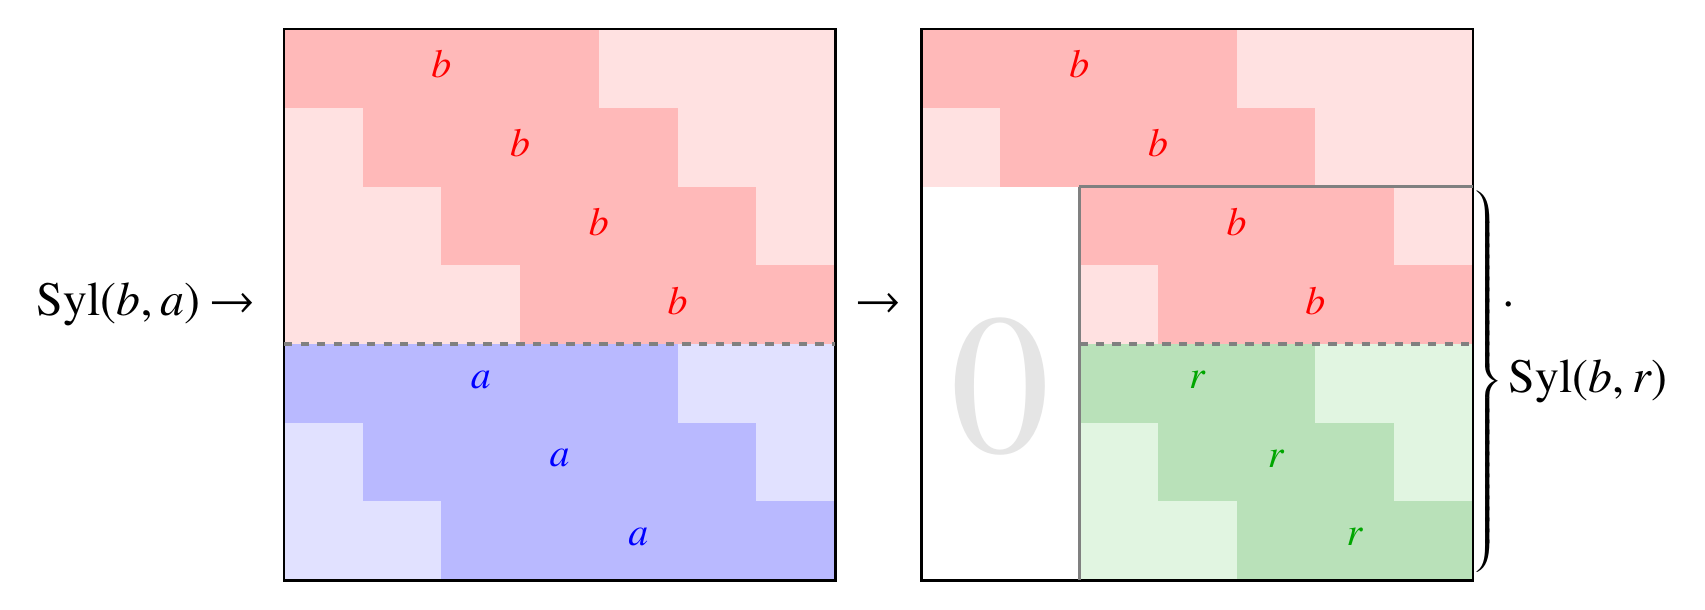
\begin{tikzpicture}[
    x=1cm,
    y=1cm,
    line cap=butt,
    every node/.style={font=\Large}
]

% Syl(b,a)
\node[font=\LARGE] at (-2.1,3.5) {$\operatorname{Syl}(b,a)$};
\node[font=\LARGE] at (-0.65,3.5) {$\to$};

% First matrix: backgrounds
\fill[lightred]  (0,3) rectangle (7,7);
\fill[lightblue] (0,0) rectangle (7,3);

% Shifted b-rows
\foreach \x/\y in {0/6,1/5,2/4,3/3}{
    \fill[rowred] (\x,\y) rectangle ++(4,1);
    \node[text=red] at (\x+2,\y+.55) {$b$};
}

% Shifted a-rows
\foreach \x/\y in {0/2,1/1,2/0}{
    \fill[rowblue] (\x,\y) rectangle ++(5,1);
    \node[text=blue] at (\x+2.5,\y+.55) {$a$};
}

% Border and dashed separation
\draw[line width=1pt] (0,0) rectangle (7,7);
\draw[gray,line width=1.2pt,dashed]
      (0,3) -- (7,3);

% Arrow between the matrices
\node[font=\LARGE] at (7.55,3.5) {$\to$};

% Second matrix
\begin{scope}[xshift=8.1cm]

% Background regions
\fill[lightred]   (0,5) rectangle (7,7);
\fill[white]      (0,0) rectangle (2,5);
\fill[lightred]   (2,3) rectangle (7,5);
\fill[lightgreen] (2,0) rectangle (7,3);

% Two remaining upper b-rows
\foreach \x/\y in {0/6,1/5}{
    \fill[rowred] (\x,\y) rectangle ++(4,1);
    \node[text=red] at (\x+2,\y+.55) {$b$};
}

% b-rows in the smaller Sylvester matrix
\foreach \x/\y in {2/4,3/3}{
    \fill[rowred] (\x,\y) rectangle ++(4,1);
    \node[text=red] at (\x+2,\y+.55) {$b$};
}

% r-rows
\foreach \x/\y in {2/2,3/1,4/0}{
    \fill[rowgreen] (\x,\y) rectangle ++(3,1);
    \node[text=green!65!black] at (\x+1.5,\y+.55) {$r$};
}

% Outer border
\draw[line width=1pt] (0,0) rectangle (7,7);

% Separation of the first two rows
% \draw[gray,line width=1pt] (0,5) -- (7,5);

% Border around the smaller matrix
\draw[gray,line width=1pt]
      (2,0) -- (2,5)
      (2,5) -- (7,5);

% Dashed separation inside Syl(b,r)
\draw[gray,line width=1.2pt,dashed]
      (2,3) -- (7,3);

% Zero block
\node[text=gray!20,scale=5] at (1,2.45) {$0$};

% Label of the smaller Sylvester matrix
\node[anchor=west, font=\LARGE] at (6.85,2.55)
      {$\left.\rule{0pt}{2.6cm}\right\}
        \operatorname{Syl}(b,r)$};

\end{scope}

\node[font=\LARGE] at (15.55,3.5) {$.$};

\end{tikzpicture}
\end{document}